\documentclass[12pt]{article}

%%%%%%%%%%%%%%%%%%%%%%%%%%%%%%%  Packages  %%%%%%%%%%%%%
\usepackage{amsmath} 
\usepackage{mathtools}
\usepackage{physics}
\usepackage{amssymb}
\usepackage{mathptmx}
\usepackage{array}

%%%%%%%%% FIGurES %%%%%%%%%%%%%%%%%%%%%%%%
\usepackage{textcomp}
\usepackage{graphicx}
\usepackage{caption} 
\usepackage{subcaption}
\usepackage{scrextend}
\usepackage{pgfgantt}
\usepackage{rotating}
\usepackage{subcaption}
\usepackage{scrextend}
\usepackage{float}
%\graphicspath{ {figures/} }
\usepackage{hyperref}
\hypersetup{colorlinks=true, citecolor=blue, linkcolor=blue}
\renewcommand{\equationautorefname}{Eq.}%
\renewcommand{\figureautorefname}{Fig.}%

%%%%%%%%%%%% LaNgUaGe %%%%%%%%%%%%%%%%%%
\usepackage[latin1]{inputenc}
\usepackage{verbatim}
\usepackage{natbib}

%%%%%%%%%%%%%%%%%% Custom maths shortcuts %%%%%%%%%
\newcommand{\ident}{\[ \mathds{1} \]}

\renewcommand{\vec}[1]{\mathbf{#1}}
\newcommand{\squeezeup}{\vspace{-2.5mm}}
\newcommand{\rtwo}{\sqrt{2}}
%\DeclarePairedDelimiter\abs{\lvert}{\rvert}%
%\newcommand{\ket}[1]{\left| #1 \right\rangle}
%\newcommand{\bra}[1]{\left\langle #1 \right|}

\usepackage{qcircuit}
\usepackage{pdflscape}
\usepackage{afterpage}
\usepackage{wrapfig}
\usepackage[a4paper]{geometry}
\usepackage{multicol}

%%%%%%%%%%%%%%%%%%%%%%%%%%%%%%%%%%%%%%%%%%%%%%%%%%%%%%%%%
\newgeometry{left=0.8in,right=0.8in,top=1in,bottom=1in}
%%%%%%%%%%%%%%%%%%%%%%%%% EnD oF pAcKaGeS %%%%%%%%%%%%%%%%

\begin{document} %WOOP WOOP!
% Title page 

    \title{Quantum Circuits for the Schur Transform}
    \author{Oliver Thomas \\[0.5em] \\ Quantum Engineering CDT \\ University of Bristol}
    \date{\today}
    \maketitle

%%%%%%%%%%%%%%%%%%%%%%%%%%%%%%%%%%%%

\section{The Schur Transform}

\textit{background.}

2004 Bacon, Chuang \& Harrow proposed a scheme for implementing the Schur transform in Poly time. 


Information processing tasks, such as classical compression gain a huge advantage implementing the process using a streaming scheme. Rather than start the compression on all the data to be sent and wait for it all to be compressed then send the data, as compression can be performed sequentially, compress part of the message and send it while compressing the next part. The Schur transform can also be thought of in this way. However, with compression it can still be useful to only compress part of the message, it is meaningless to perform only part of the Schur transform which suggests there may be a more optimal scheme opposed to streaming for implementing the Schur transform.      

This report is structured as follows,   

There are two distinct ways of performing the Schur transform on $n$ qubits, it can either be built up from coupling
all $n$ qubits together in a single iteration which we call the spatial multiplexed approach. The other approach is 
performing Clebsch-Gordan (CG) transforms on the $n$ qubits one at a time which we call the temporal multiplexed 
approach.  





\section{Streaming Scheme}

Information processing tasks, such as classical compression gain a huge advantage implementing the process using a streaming scheme. Rather than start the compression on all the data to be sent and wait for it all to be compressed then send the data, as compression can be performed sequentially, compress part of the message and send it while compressing the next part. The Schur transform can also be thought of in this way. However, with compression it can still be useful to only compress part of the message, it is meaningless to perform only part of the Schur transform which suggests there may be a more optimal scheme opposed to streaming for implementing the Schur transform.      

The streaming Schur transform is described in \autoref{fig:stream},

\begin{figure}[h!]
\centering
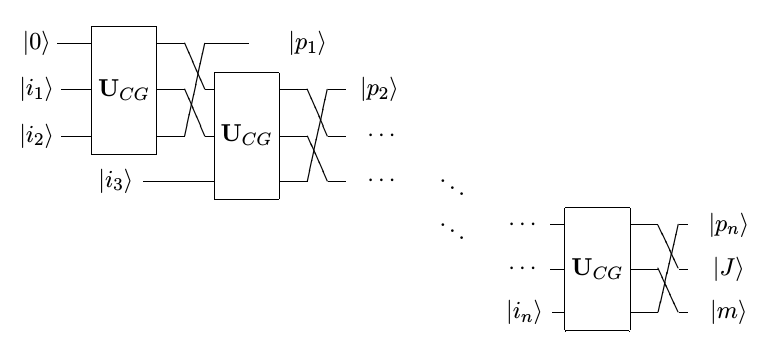
\includegraphics[width=0.6\textwidth]{schurcascade.png}
\caption{Streaming structure where the Schur transform is built up from consecutive Clebsch-Gordan transforms \cite{bacon2006efficient}.}
\label{fig:stream}
\end{figure}

The aim of this report is to look at whether it is possible to achieve a log decrease in time by instead of coupling 1 qubit in at a time to the $J$ \& $M$ registers, to pairing the couplings up in a \textbf{binary tree?} technique. To investigate the problem we look at how the complexity of performing the Clebsch-Gordan transform scales moving from coupling a single qubit to an arbitrary $J \& M$ to coupling arbitrary $J \& M$ registers together. looking at the pairing approach there is a symmetry in the fact that the max range of $J \& M$ values will be the same within each pairing which will help simplify the problem compared to any arbitrary $J \& M$ values.

For the streaming scheme the $U_{CG}$ block can be chosen so that it contains all of the gates for upto the n-th qubit meaning the same block can be repeated. 
Where the $U_{CG}$ is the Clebsch-Gordan transform between the $J$ \& $M$ registers and the k-th qubit $\ket{i_k}$.

\begin{figure}[h!]
\centering
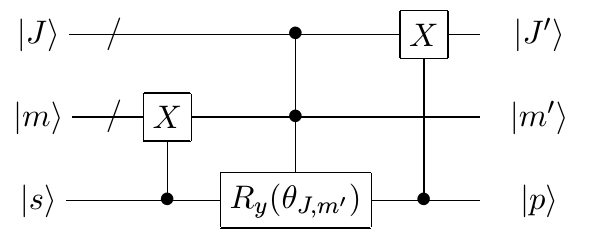
\includegraphics[width=0.6\textwidth]{genaddercirc.png}
\caption{$U_{CG}$ block, Qadder, controlled rotation, Qadder \cite{bacon2006efficient}.}
\label{fig:ucg}
\end{figure}

The controlled Rotation matrix, $R_y(\theta_{J,m'})$ \autoref{fig:stream} is the Clebsch-Gordan coefficients for coupling 1 qubit sequentially, given by,
\begin{align}
\begin{split}
R_y(\theta_{J,m'})=
\begin{bmatrix}
\cos(\theta_{J,m'}) &-\sin(\theta_{J,m'}) \\
\sin(\theta_{J,m'}) & \cos(\theta_{J,m'}) \\
\end{bmatrix}
\end{split}
=
\begin{split}
\frac{1}{\sqrt{2J+1}}
\begin{bmatrix}
\sqrt{J+\frac{1}{2}+m'} &-\sqrt{J+\frac{1}{2}-m'} \\
\sqrt{J+\frac{1}{2}-m'} & \sqrt{J+\frac{1}{2}+m'} \\
\end{bmatrix}
\end{split}
\label{eq:rotmatrix}
\end{align}

Where primed variables means after the angular momentum addition so $J$ is the total J that the spin is coupling to, the system will have $J'$ total angular momentum after the coupling. $m$ is the z component of the system before and $m'$ is the total z component after the coupling.

To build this circuit the rotation matrix, $R_y(\theta_{J,m'})$ needs to be calculated using \autoref{eq:rotmatrix}, values here \autoref{eq:rvalues}, and a function to update the $\ket{m}$ and $\ket{J}$ registers is needed. Updating the registers can be implemented relatively simply using the coherent (meaning the registers are allowed to be in superpositions) equivalent of the digital full adders and subtractors. The complexity now has been reduced to implementing the Clebsch-Gordan transform, $U_{CG}$.

\section{Implementing the Clebsch-Gordan Transform}

The vanilla transform directly maps the computation basis states to a labeling of J and M values. The vanilla approach of calculating the CG coefficients and finding a gate decomposition does not scale well. A better approach is to use a scheme explicitly storing the values of J \& M in registers.

The streaming scheme uses temporal multiplexing to perform the Schur transform in polynomial time if a recursive streaming scheme is used \cite{bacon2007quantum}.

%%%%%%%%%%%%%% 2 qubits
\section{Spatially multiplexed Clebsch-Gordan transform for 2 qubits}

The Clebsch-Gordan transform is a basis transformation into the Schur basis. The transform for 2 qubits is given by,
\begin{subequations}
\begin{align}
\begin{split}
&\ket{J=1, M=+1} = \ket{00} \\
&\ket{J=1, M=\;\;\;0} = \frac{1}{\sqrt{2}}(\ket{01} + \ket{10}) \\
&\ket{J=1, M=-1} = \ket{11} \\
\end{split}\\
\begin{split}
&\ket{J=0, M=\;\;\;0} = \frac{1}{\sqrt{2}}(\ket{01} - \ket{10})\\
\end{split}
\end{align}
\end{subequations}

Throughout the encoding $\ket{0}=+1/2$, $\ket{1}=-1/2$ is used unless stated otherwise.

The transform expressed as a matrix is,
\begin{align}
\begin{bmatrix}
1 & 0 & 0 & 0 \\
0 & \frac{1}{\sqrt{2}} & \frac{1}{\sqrt{2}} & 0 \\
0 & 0 & 0 & 1 \\
0 & \frac{1}{\sqrt{2}} & -\frac{1}{\sqrt{2}} & 0 \\
\end{bmatrix}
\begin{bmatrix}
\ket{00} \\
\ket{01} \\
\ket{10} \\
\ket{11} \\ 
\end{bmatrix}
= \text{(spin labeling)}
\begin{bmatrix}
\ket{00} \\
\frac{1}{\sqrt{2}}(\ket{01} + \ket{10}) \\
\ket{11} \\
\frac{1}{\sqrt{2}}(\ket{01} - \ket{10}) \\ 
\end{bmatrix}
=
\begin{bmatrix}
\ket{J=1, M=1} \\
\ket{J=1, M=0} \\
\ket{J=1, M=-1} \\
\ket{J=0, M=0} \\ 
\end{bmatrix}
\end{align}

Which can be implemented in a circuit as,
%%%%%%%%% circuit 1 
\begin{figure}[h]
\begin{align}
\Qcircuit @C=0.5cm @R=0.7cm{
%1
&\lstick{S_1} &\gate{H} &\ctrl{1} &\qw \\
%0
&\lstick{S_0} &\ctrl{-1} &\targ &\qw \\
}
\end{align}
\caption{Schur transform for 2 qubits}
\label{cir:vanilla2}
\end{figure}

Circuit for Clebsch-Gordan transform \autoref{cir:vanilla2} contains 2 gates. As two-qubit (entangling) gates are much more expensive to perform compared to single qubit gates, the cost of the circuits discussed here will all be given in terms of the number of two-qubit gates. 

\subsection{Clebsch-Gordan coefficients for 3 qubits}

The CG coefficients for three qubits are no multiplicities of 4 for J=3/2 and 2 multiplicities of 2 for J=1/2  \autoref{eq:3cgcoeff}. The multiplicities, P are defined as $J'-J$ the new J value minus the previous J value, the number of 1s in a P string is the number of multiplicities for that J value.

%%%%%%%%%%%%%%% vanilla basis %%%%%%%%%%%%%%%%%%5

The matrix for the transform which takes the computational basis to the spin basis is,
\begin{align}
\begin{bmatrix}
1 &0 &0 &0 &0 &0 &0 &0 \\
0 &\sqrt{\frac{1}{3}} &\sqrt{\frac{1}{3}} &0 &\sqrt{\frac{1}{3}} &0 &0 &0\\
0 &0 &0 &\sqrt{\frac{1}{3}} &0 &\sqrt{\frac{1}{3}} &\sqrt{\frac{1}{3}} &0 \\
0 &0 &0 &0 &0 &0 &0 &1 \\
0 &\sqrt{\frac{2}{3}} &-\sqrt{\frac{1}{6}} &0 &-\sqrt{\frac{1}{6}} &0 &0 &0\\
0 &0 &0 &\sqrt{\frac{1}{6}} &0 &\sqrt{\frac{1}{6}} &-\sqrt{\frac{2}{3}} &0 \\
0 &0 &\frac{1}{\rtwo} &0 &-\frac{1}{\rtwo} &0 &0 &0 \\
0 &0 &0 &\frac{1}{\rtwo} &0 &-\frac{1}{\rtwo} &0 &0 \\
\end{bmatrix}
%
\begin{bmatrix}
000 \\
001 \\
010 \\
011 \\
100 \\
101 \\
110 \\
111 \\
\end{bmatrix}
=
\begin{bmatrix}
\ket{J=3/2, M=3/2} \\
\ket{J=3/2, M=1/2} \\
\ket{J=3/2, M=-1/2} \\
\ket{J=3/2, M=-3/2} \\ 
\hline
\ket{J=1/2, M=1/2, P=0} \\
\ket{J=1/2, M=-1/2, P=0} \\
\hline
\ket{J=1/2, M=1/2, P=1} \\
\ket{J=1/2, M=-1/2, P=1} \\ 
\end{bmatrix}
\label{eq:3qubitcg}
\end{align}

The decomposition scheme for the n-qubit case could take at most $2^{n-1}(2^n-1)$ $C^{n-1}U$ gates \cite{li2013decomposition}, where $C^{n-1}U$ means a unitary acting on 1 qubit controlled on the other n-1 qubits. For 3 qubits this upper bound is 128 $C^2U$ gates. It has been shown that in terms of gate count, $C^nU \sim 5 C^{n-1}V$ where $U \& V$ are unitaries \cite{barenco1995elementary}. This means the maximum two-qubit gates needed would be 140 $CU$ gates.

The decomposition of the 3 qubit CG transform was performed using the Givens rotation method for unitary decomposition into a gate-set. The matrix \autoref{eq:3qubitcg} can be expressed as a product of 19 $C^2U$ gates (control-control-unitaries) which is $\sim$80 $CU$ gates. 

There are multiple ways of writing the spin basis, there is the traditional CG coefficients and there is also what is referred to here as the phase encoding \autoref{eq:phaseencode}. The phase encoded transform matrix will have a different decomposition as the shape of the matrix is different to the regular encoding. 


\begin{comment}
%%%%%%%%%%%%%%%%%%%%%%%%%%%% pt 2 %%%%%%%%%%%%%%%%%%%%%%%
\begin{table}[h]
\centering
\begin{tabular}{ |c | c| } 
\hline
%%%%%%%%%%%%%%%%% J=3/2 from j=1, j=1/2  p=000 %%%%%%%%%%%%%%%
$J=\frac{3}{2}$ (P=000 j=1/2, j=1, j=3/2) &$S=\frac{3}{2}$ \\
\hline  
 $000$ &$M=\frac{3}{2}$ \\
 $\sqrt{\frac{1}{3}}(001+010+100)$  &$M=\frac{1}{2}$ \\ 
 $\sqrt{\frac{1}{3}}(110+011+101)$  &$M=-\frac{1}{2}$ \\
 $111$ &$M=-\frac{3}{2}$ \\
\hline
%%%%%%%%%%%%%%%%% J=1/2 from j=1, j=1/2 p=001 %%%%%%%%%%%%%%%%%%
$J=\frac{1}{2}$ (P=001 j=1/2, j=1, j=1/2) &$S=\frac{1}{2}$ \\
\hline
 $\sqrt{\frac{2}{3}}(001) - \sqrt{\frac{1}{6}}(010+100)$  &$M=\frac{1}{2}$ \\ 
 $-\sqrt{\frac{2}{3}}(110) + \sqrt{\frac{1}{6}}(011+101)$  &$M=-\frac{1}{2}$ \\ 
\hline 
%%%%%%%%%%%%%%%%% J=1/2 from j=0, j=1/2 p=010 %%%%%%%%%%%%%%%%
$J=\frac{1}{2}$ (P=010 j=1/2, j=0, j=1/2) &$S=\frac{1}{2}$ \\
\hline
 $\frac{1}{\rtwo} (010-100)$ &$M=\frac{1}{2}$\\
 $\frac{1}{\rtwo} (011-101)$ &$M=-\frac{1}{2}$ \\ 
\hline 
\end{tabular}
\caption{J \& M values for 3 qubits using encoding 0=spin up, 1=spin down}
\label{fig:tab1}
\end{table}
\end{comment}



\begin{comment}
\begin{table}[h]
\centering
\begin{tabular}{ |c | c| } 
\hline
$J=\frac{3}{2}$ &$S=\frac{3}{2}$ \\
\hline  
 $000$ &$M=\frac{3}{2}$ \\
 $\sqrt{\frac{1}{3}}(001+010+100)$  &$M=\frac{1}{2}$ \\ 
 $\sqrt{\frac{1}{3}}(110+011+101)$  &$M=-\frac{1}{2}$ \\
 $111$ &$M=-\frac{3}{2}$ \\
\hline
$J=\frac{1}{2}, P=0$ &$S=\frac{1}{2}$ \\
\hline
 $\frac{1}{\sqrt{3}} (e^{2\pi i/3}001+e^{4\pi i/3}010+100)$ &$M=\frac{1}{2}$\\
 $\frac{1}{\sqrt{3}} (e^{2\pi i/3}011+e^{4\pi i/3}101+110)$ &$M=-\frac{1}{2}$ \\ 
\hline 
$J=\frac{1}{2}, P=1$ &$S=\frac{1}{2}$ \\
\hline
 $\frac{1}{\sqrt{3}} (e^{2\pi i/3}001+e^{4\pi i/3}010+100)$ &$M=\frac{1}{2}$\\
 $\frac{1}{\sqrt{3}} (e^{4\pi i/3}011+e^{2\pi i/3}101+110)$ &$M=-\frac{1}{2}$ \\ 
\hline 
\end{tabular}
\caption{Schur transform with Phase encoding?}
\end{table}
\end{comment}



%%%%%%%%%%%%%%%%%%%%%%%%%%%%%%%%%%%%%%%%%%%%%%%%%%%%%%%%%%%%%%%%%%%%%%%%%%%%%%%%%%%%%%%%%

\subsection{Circuit for 3 qubit transform}

\Qcircuit @C=0.7cm @R=0.7cm {
&\qw \\
}

See online \cite{githubot561} for Fortran code which implements the Givens rotation method to give the 19 $C^2U$ gate decomposition. The majority of the gates are CNOT gates. This is mainly due to the re-ordering of the basis and is similar to the quantum Fourier transform (QFT). The QFT produces the output in reverse qubit order the actual number of gates required to do the transform is massively reduced. The overhead calculated here is due to the rearranging of the basis. This means that depending on what the transform is used the transform could be computed with less gates. For example, if the transform was only used to check if the state was in a particular J block but didn't need to know the specific M value the order afterwards wouldn't be as important reducing the CNOTs needed.


\subsection{4 Qubit CG coefficients}

The CG coefficients for four qubits contains 16 terms, 5 for J=2, 3 multiplicities of 3 for J=1, 2 multiplicities of 1 for J=0. The equations are given in \autoref{eq:4qubitcg}. In the J=1 case there are 3 acceptable bit strings, 0001, 0010, 0100 meaning there are 3 multiplicities present. 

The decomposition scheme for the 4 qubit case could take at most $2^{n-1}(2^n-1)$ $C^{n-1}U$ gates \cite{li2013decomposition}, where n is 4 and. For 4 qubits this upper bound is 120 $C^3U$ gates which could be up to $\sim 3000$ $CU$ gates. In reality it will be much fewer gates as the matrix is sparse, however this suggests a different approach was needed.

\begin{comment}

{\renewcommand{\arraystretch}{1.5}
\begin{tabular}{ |c | c| } 
\hline
\hline
%%%%%%%%%%%%%% J=2 from j=3/2, j=1, j=1/2 p=0000 %%%%%%%%%%%%%%%%%%%
$J'=2$, (P=0000 j=1/2, j=1, j=3/2, j=2)&$S=2$ \\
\hline  
 $0000$ &$M=2$ \\
 $\frac{1}{2}(0001+0010+0100+1000)$  &$M=1$ \\ 
 $\sqrt{\frac{1}{6}}(0011+0101+1001+1100+1010+0110)$  &$M=0$ \\
 $\frac{1}{2}(1110+1101+1011+0111)$  &$M=-1$ \\ 
 $1111$ &$M=-2$ \\
\hline
\hline
%%%%%%%%%%%%%%% J=1 from j=3/2, j=1, j=1/2 p=0001 %%%%%%%%%%%%%%%%%%%
$J'=1$, (P=0001 j=1/2, j=1, j=3/2, j=1) &$S=1$ \\
\hline  
 $\sqrt{\frac{3}{4}}(0001) - \sqrt{\frac{1}{12}}(0010+0100+1000)$  &$M=1$ \\ 
 $\sqrt{\frac{1}{6}}((0011+0101+1001)-(1100+1010+0110))$  &$M=0$ \\
 $-\sqrt{\frac{3}{4}}(1110)+\sqrt{\frac{1}{12}}(1101+1011+0111)$  &$M=-1$ \\ 
\hline
\hline
%%%%%%%%%%%%%   J=1 from j=1/2, j=1, j=1/2 p=0010 %%%%%%%%%%%%%5
$J'=1$, (P=0010 j=1/2, j=1, j=1/2, j=1) &$S=1$ \\
\hline  
 $\sqrt{\frac{2}{3}}(0010) - \sqrt{\frac{1}{6}}(0100+1000)$  &$M=1$ \\ 
 $\sqrt{\frac{1}{3}}(0011-1100) + \sqrt{\frac{1}{12}}(0110+1010-0101-1001)$  &$M=0$ \\
 $-\sqrt{\frac{2}{3}}(1101)+\sqrt{\frac{1}{6}}(1011+0111)$  &$M=-1$ \\ 
\hline
\hline
%%%%%%%%%%% J=1 from j=1/2, j=0, j=1/2 p=0100 %%%%%%%%%%%%%%%%%%
$J'=1$, (P=0100 j=1/2, j=0, j=1/2, j=1) &$S=1$ \\
\hline  
 $\sqrt{\frac{1}{2}}(0100-1000)$  &$M=1$ \\ 
 $\frac{1}{2}(0101-1001+0110-1010)$  &$M=0$ \\
 $-\sqrt{\frac{1}{2}}(0111-1011)$  &$M=-1$ \\ 
\hline
\hline
%%%%%%%%%%%%%%%%% J=0 from j=1/2, j=1, j=1/2 p=0011 %%%%%%%%%%%%%%%%%%
$J'=0$, (P=0011 j=1/2, j=1, j=1/2, j=0)  &$S=0$ \\
\hline  
 $\sqrt{\frac{1}{3}}(0011+1100)-\sqrt{\frac{1}{12}}(0101+1001+0110+1010)$  &$M=0$ \\ 
\hline
\hline
%%%%%%%%%%%%%%%%% J=0 from j=1/2, j=0, j=1/2 p=0101 %%%%%%%%%%%%%%%%
$J'=0$, (P=0101 j=1/2, j=0, j=1/2, j=0) &$S=0$ \\
\hline  
 $\frac{1}{2}(0101-1001-0110+1010)$  &$M=0$ \\
\hline
\hline
%%%%%%%%%%%%%%%%%%%%%%%%%%%%%%%%%%%%%%%%%%%%%%%%%%%%%%%%
\end{tabular}
}

\end{comment}


\subsection{Registering J \& M explicitly \autoref{cir:spatialmulti2}, \autoref{cir:minspatialmult}}

The registered circuit, which takes in two qubits can be constructed from 11 gates if the m register is not compressed. The spatially multiplexed minimal gate explicit J \& M 2 qubit transform is shown in \autoref{cir:minspatialmult} which contains 11 two-qubit gates. Another CNOT can be added to compress the M' register, which means using the same values for M'=0, see \autoref{cir:spatialmulti2} for the 12 two-qubit gate circuit.

This spatial multiplexing approach only stores the final output values of the $J$ \& $M$ registers. 


\section{General circuit for the Quantum Schur transform \autoref{cir:genstreaming}}

Circuit uses the encoding for $\ket{S} : \ket{0} \mapsto Spin = +\frac{1}{2}, \ket{1} \mapsto Spin = -\frac{1}{2}$ and the same for $\ket{P}$. 

The circuit adds the value of the spin to be added, $\ket{S}$, to the M register to calculate the M' register value. This is done by implementing the quantum reversible equivalent to the digital full adder. 

\begin{wraptable}{r}{5.5cm}
\begin{tabular}{ |c c c|c| }
\hline
 $J_2$ &$J_1$ &$J_0$ &J \\
 \hline
 0 &0 &0 &0 \\ 
 0 &0 &1 &$\frac{1}{2}$ \\ 
 0 &1 &0 &1 \\ 
 0 &1 &1 &$\frac{3}{2}$ \\ 
 \hline 
 1 &0 &0 &-2 \\ 
 1 &0 &1 &-$\frac{3}{2}$ \\ 
 1 &1 &0 &-1 \\ 
 1 &1 &1 &-$\frac{1}{2}$ \\  
 \hline 
\end{tabular}
\quad
\begin{tabular}{ |c c c|c| } 
\hline
 $m_2$ &$m_1$ &$m_0$ &M \\
 \hline
 0 &0 &0 &0 \\ 
 0 &0 &1 &$\frac{1}{2}$ \\ 
 0 &1 &0 &1 \\ 
 0 &1 &1 &$\frac{3}{2}$ \\ 
 \hline 
 1 &0 &0 &-2 \\ 
 1 &0 &1 &-$\frac{3}{2}$ \\ 
 1 &1 &0 &-1 \\ 
 1 &1 &1 &-$\frac{1}{2}$ \\  
 \hline
\end{tabular}
\caption{Tables giving binary Two's complement encoding to spin values of the M and J registers}
\label{tab:encoding}
\end{wraptable}

The case where $\ket{S} = \ket{0}$ means the spin is $+\frac{1}{2}$ so to add $\frac{1}{2}$ to M, 1 is added to the $m_0$ qubit. The first Quantum Adder (QAdd) uses Toffoli gates controlled on $\ket{s}=\ket{0}$ (denoted by the white control circle) with the current $m_0$ value and $C_0$ (an ancilla carry). This ensures that the case when $m_0 = 1$ and 1 is added to it, $m_0$ goes to 0 and $m_1$ is increased using the carry as $001+1=010$. The rest of the QAdd stages then just check the carry of the previous qubit to complete to M $+ \frac{1}{2}$ addition as $\ket{S} = \ket{0}$ does not trigger any of the rest of the control gates.

The case where $\ket{S} = \ket{1}$ means the spin is $-\frac{1}{2}$ we do M $-\frac{1}{2}$ which is done by adding the binary string for $-\frac{1}{2}$ which is the all 1's string, 111. This time the very first QAdd does not trigger and $\ket{s}$ is then added to all of the bits of M using C-NOT gates with carries to check for overflow. 

The Unitary is then performed on $\ket{S}$ depending on the values of the newly calculated M' and J registers using $R_y(\theta_{J,m'})$ \autoref{eq:rotmatrix}. The J register is then updated to J' by adding the value of $\ket{P}$ to J using the QAdd sequence of gates.

To add the second qubit in the values of J' and M' are passed in as the initial register values. It is easy to extend this to many qubits being streamed in one at a time by carefully conditioning the controls on the unitaries, I think in the general case you need at most N controls for coupling up to N qubits in one at a time. The circuit written here has redundancy in the Identity and ZX gates appearing twice which is shown in the circuit for completeness\autoref{cir:genstreaming}. 

\section{Reduced general gate circuit for up to the 2 qubit Schur transform \autoref{cir:tempmultistream}}

Where $V$ is the phase gate, 
$ V = \begin{bmatrix}
1 & 0 \\
0 & i \\
\end{bmatrix} $
, $V^{\dag}V = I$ and $V^2 = Z$. $V$ is used here to expand the double controlled Toffoli gate into single control gates in the quantum adder subroutine.

The $W$ gate, $W^2 = HX$ with $W^{\dag} = I$, is used to expand the $HX$ gate into single control gates in the spin transform region. 

The circuit checks that if ($m_1$ XNOR $m_0$) AND ($m_0$ XOR $S_0$) and will then change $m_2$. Then $m_1$ is updated using $m_1 = m_0$ XOR $S_0$. $m_0$ is always incremented by 1, if $\ket{S} = \ket{0}$ increment only $m_0$ by 1 corresponding to adding $\frac{1}{2}$ to the $M$ register. $\ket{S} = \ket{1}$ corresponds to subtracting $\frac{1}{2}$ from the $M$ register by adding the string 111 bitwise to $M$. 
 
For the most positive values of $M$ the Identity is performed on the spin corresponding to the strings $M=001 (J=\frac{1}{2}, M' = \frac{1}{2})$ for the first spin and $M=010 (J=1, M'=1) $ for the second coupled in spins. 

The most negative values of $M$ performs $XZ \ket{S}$ corresponding to the strings $M=111 (J=\frac{1}{2}, M'=-\frac{1}{2})$ for the first spin and $M=110 (J=1, M'=-1)$ for the second spin.

If $M=000 (J=0, M'=0)$ do $XH \ket{S}$ \autoref{cir:tempmultistream}.  


%%%%%%%%%%%%
\bibliographystyle{unsrt}
\bibliography{references}

\newpage
\appendix
\section{Appendix: Maths}

\subsection{3 Qubit transformation}

\begin{subequations}
\begin{align}
\intertext{ This is the J=3/2 block}
\begin{split}
&\ket{J=3/2, M=+3/2, P=000} = \ket{000} \\
&\ket{J=3/2, M=+1/2, P=000} = \sqrt{\frac{1}{3}}(\ket{001}+\ket{010}+\ket{100}) \\
&\ket{J=3/2, M=-1/2, P=000} = \sqrt{\frac{1}{3}}(\ket{110}+\ket{011}+\ket{101}) \\
&\ket{J=3/2, M=-3/2, P=000} = \ket{111} \\ 
\end{split} \\
\intertext{ This is the J=1/2 block from J=1, multiplicity zero}
\begin{split}
&\ket{J=1/2, M=+1/2, P=001} =+\sqrt{\frac{2}{3}}\ket{001} - \sqrt{\frac{1}{6}}(\ket{010}+\ket{100}) \\
&\ket{J=1/2, M=-1/2, P=001} =-\sqrt{\frac{2}{3}}\ket{110} + \sqrt{\frac{1}{6}}(\ket{011}+\ket{101}) \\ 
\end{split} \\
\intertext{ This is the J=1/2 block from J=0, multiplicity one}
\begin{split}
&\ket{J=1/2, M=+1/2, P=010} = \frac{1}{\rtwo} (\ket{010}-\ket{100})\\
&\ket{J=1/2, M=-1/2, P=010} = \frac{1}{\rtwo} (\ket{011}-\ket{101})\\
\end{split} 
\label{eq:3cgcoeff}
\end{align}
\end{subequations}

The CG transform for 3 qubits \autoref{eq:3qubitcg} can be rearranged to a block diagonal form which looks like it could be implemented in a circuit.
\begin{align}
\begin{bmatrix}
1 &0 &0 &0 &0 &0 &0 &0 \\
0 &\sqrt{\frac{2}{3}} &-\sqrt{\frac{1}{6}} &-\sqrt{\frac{1}{6}} &0 &0 &0 &0\\
0 &\sqrt{\frac{1}{3}} &\sqrt{\frac{1}{3}} &\sqrt{\frac{1}{3}} &0 &0 &0 &0\\
0 &0 &\frac{1}{\rtwo} &-\frac{1}{\rtwo} &0 &0 &0 &0 \\
0 &0 &0 &0 &\frac{1}{\rtwo} &-\frac{1}{\rtwo} &0 &0 \\
0 &0 &0 &0 &\sqrt{\frac{1}{3}} &\sqrt{\frac{1}{3}} &\sqrt{\frac{1}{3}} &0 \\
0 &0 &0 &0 &\sqrt{\frac{1}{6}} &\sqrt{\frac{1}{6}} &-\sqrt{\frac{2}{3}} &0 \\
0 &0 &0 &0 &0 &0 &0 &1 \\
\end{bmatrix}
\begin{bmatrix}
000 \\
001 \\
010 \\
100 \\
011 \\
101 \\
110 \\
111 \\
\end{bmatrix}
\end{align}

%%%%%%%%%%%%%%%%%%% 3 Qubits Phase encoding
\subsection{3 Qubit phase encoding}

\begin{subequations}
\begin{align}
\intertext{ This is the J=3/2 block}
\begin{split}
&\ket{J=3/2, M=+3/2, P=000} = \ket{000} \\
&\ket{J=3/2, M=+1/2, P=000} = \sqrt{\frac{1}{3}}(\ket{001}+\ket{010}+\ket{100}) \\
&\ket{J=3/2, M=-1/2, P=000} = \sqrt{\frac{1}{3}}(\ket{110}+\ket{011}+\ket{101}) \\
&\ket{J=3/2, M=-3/2, P=000} = \ket{111} \\ 
\end{split} \\
%\vspace{3pt} \nonumber\\
\intertext{ This is the J=1/2 block from J=1, multiplicity zero}
\begin{split}
&\ket{J=1/2, M=+1/2, P=001} = \frac{1}{\sqrt{3}} (\ket{001} + e^{2\pi i/3}\ket{100}+e^{4\pi i/3}\ket{010}) \\
&\ket{J=1/2, M=-1/2, P=001} =\frac{1}{\sqrt{3}} (\ket{011} + e^{2\pi i/3} \ket{101}+e^{4\pi i/3}\ket{110}) \\ 
\end{split} \\
%\vspace{3pt} \nonumber \\
\intertext{ This is the J=1/2 block from J=0, multiplicity one}
\begin{split}
&\ket{J=1/2, M=+1/2, P=010} = \frac{1}{\sqrt{3}} (\ket{001} + e^{4\pi i/3}\ket{100}+e^{2\pi i/3}\ket{010}) \\
&\ket{J=1/2, M=-1/2, P=010} =\frac{1}{\sqrt{3}} (\ket{011} + e^{4\pi i/3}\ket{101} +e^{2\pi i/3}\ket{110})\\
\end{split} 
\end{align}
\end{subequations}

The phase encoding matrix is given by,
% table pt 2 phase encoding

\begin{align}
\frac{1}{\sqrt{3}}
\begin{bmatrix}
\sqrt{3} &0 &0 &0 &0 &0 &0 &0 \\
0 &1 &1 &0 &1 &0 &0 &0 \\
0 &0 &0 &1 &0 &1 &1 &0\\
0 &0 &0 &0 &0 &0 &0 &\sqrt{3} \\
0 &e^{2\pi i/3} &e^{4\pi i/3} &0 &1 &0 &0 &0 \\
0 &0 &0 &e^{2\pi i/3} &0 &e^{4\pi i/3} &1 &0 \\
0 &e^{4\pi i/3} &e^{2\pi i/3} &0 &1 &0 &0 &0\\
0 &0 &0 &e^{4\pi i/3} &0 &e^{2\pi i/3} &1 &0 \\
\end{bmatrix}
\begin{bmatrix}
000 \\
001 \\
010 \\
011 \\
100 \\
101 \\
110 \\
111 \\
\end{bmatrix}
=
\begin{bmatrix}
\ket{J=3/2, M=3/2} \\
\ket{J=3/2, M=1/2} \\
\ket{J=3/2, M=-1/2} \\
\ket{J=3/2, M=-3/2} \\ 
\hline
\ket{J=1/2, M=1/2, P=0} \\
\ket{J=1/2, M=-1/2, P=0} \\
\hline
\ket{J=1/2, M=1/2, P=1} \\
\ket{J=1/2, M=-1/2, P=1} \\ 
\end{bmatrix}
%\end{align}
\label{eq:phaseencode}
\end{align}

Where this is a different form to the other basis for 3 qubits \autoref{eq:3qubitcg}.

\subsection{4 Qubit CG coefficients}
%%%%%%%%%%%%%%%%%%%%%%%%%%%%% 4 Qubit CG
\begin{subequations}
\begin{align}
%%%%%%%%%%%%%%%%%%%% J=2
\intertext{The J=2 block, P=0000, (J=1/2, J=1, J=3/2, J=2)}
\begin{split}
&\ket{J=2, M=+2, P=0000} = \ket{0000} \\
&\ket{J=2, M=+1, P=0000} = \frac{1}{2}(\ket{0001}+\ket{0010}+\ket{0100}+\ket{1000}) \\
&\ket{J=2, M=\;\;\;0, P=0000} = \sqrt{\frac{1}{6}}(\ket{0011}+\ket{0101}+\ket{1001}+\ket{1100}+\ket{1010}+\ket{0110}) \\
&\ket{J=2, M=-1, P=0000} = \frac{1}{2}(\ket{1110}+\ket{1101}+\ket{1011}+\ket{0111}) \\
&\ket{J=2, M=-2, P=0000} = \ket{1111} \\ 
\end{split} \\
%%%%%%%%%%%%%%%%%%% J=1 (0)
\vspace{5pt} \nonumber \\
\intertext{The J=1 (0) block, P=0001, (J=1/2, J=1, J=3/2, J=1)}
\begin{split}
&\ket{J=1, M=+1, P=0001} =+\sqrt{\frac{3}{4}}\ket{0001} - \sqrt{\frac{1}{12}}(\ket{0010}+\ket{0100}+\ket{1000}) \\
&\ket{J=1, M=\;\;\;0, P=0001} = \sqrt{\frac{1}{6}}(\ket{0011}+\ket{0101}+\ket{1001}-\ket{1100}-\ket{1010}-\ket{0110}) \\
&\ket{J=1, M=-1, P=0001} =-\sqrt{\frac{3}{4}}\ket{1110} + \sqrt{\frac{1}{12}}(\ket{1101}+\ket{1011}+\ket{0111}) \\ 
\end{split} \\
%%%%%%%%%%%%%%%%%%% J=1 (1)
\vspace{3pt} \nonumber \\
\intertext{The J=1 (1) block, P=0010, (J=1/2, J=1, J=1/2, J=1)}
\begin{split}
&\ket{J=1, M=+1, P=0010} =+\sqrt{\frac{2}{3}}\ket{0010} - \sqrt{\frac{1}{6}}(\ket{0100}+\ket{1000}) \\
&\ket{J=1, M=\;\;\;0, P=0010} = \sqrt{\frac{1}{3}}(\ket{0011}-\ket{1100}) + \sqrt{\frac{1}{12}}(\ket{0110}+\ket{1010}-\ket{0101}-\ket{1001})\\
&\ket{J=1, M=-1, P=0010} =-\sqrt{\frac{2}{3}}\ket{1101}+\sqrt{\frac{1}{6}}(\ket{1011}+\ket{0111})\\ 
\end{split} \\
%%%%%%%%%%%%%%%%%% J=1 (2)
\vspace{3pt} \nonumber \\
\intertext{The J=1 (2) block, P=0100, (J=1/2, J=0, J=1/2, J=1)}
\begin{split}
&\ket{J=1, M=+1, P=0100} =+\sqrt{\frac{1}{2}}(\ket{0100}-\ket{1000}) \\
&\ket{J=1, M=\;\;\;0, P=0100} = \frac{1}{2}(\ket{0101}-\ket{1001}+\ket{0110}-\ket{1010}) \\
&\ket{J=1, M=-1, P=0100} =-\sqrt{\frac{1}{2}}(\ket{0111}-\ket{1011})\\ 
\end{split} \\
%%%%%%%%%%%%%%%%% J=0 (0)
\vspace{5pt} \nonumber \\
\intertext{The J=0 block, P=0011, (J=1/2, J=1, J=1/2, J=0)}
\begin{split}
&\ket{J=0, M=0, P=0011} = \sqrt{\frac{1}{3}}(\ket{0011}+\ket{1100})-\sqrt{\frac{1}{12}}(\ket{0101}+\ket{1001}+\ket{0110}+\ket{1010}) \\
\end{split} 
%%%%%%%%%%%%%%%%% J=0 (1)
\vspace{3pt} \\
\intertext{The J=0 block, P=0101, (J=1/2, J=0, J=1/2, J=0)}
\begin{split}
&\ket{J=0, M=0, P=0101} = \frac{1}{2}(\ket{0101}-\ket{1001}-\ket{0110}+\ket{1010}) \\
\end{split} 
\label{eq:4qubitcg}
\end{align}
\end{subequations}
%%%%%%%%%%%%%%%%%%%%%%%%%%%%%%%%%%%%%%%%%%%%%%%%%%%%%%%%%%%%%%%%%%%%%%%%%%%%%%%%%%%%%%%%%%%%%%%%%%

\subsection{Rotation matrix for J \& M values}
%%%%%%%%%%%%%%%%%%%%%%%%%%%%%%%%%%%
\begin{subequations}
\begin{align}
%%%%%%%%%%%%%%%%% J=0 (0)
%\vspace{5pt} \nonumber \\
\intertext{J=0 values}
\begin{split}
&\ket{J=0, M'=+1/2} = R = I \\
&\ket{J=0, M'=-1/2} = R = XZ \\
\end{split} \\ 
%%%%%%%%%%%%%%%% J=1/2
%\vspace{5pt} \nonumber \\
\intertext{J=1/2 values}
\begin{split}
&\ket{J=1/2, M'=+1} = R = I \\
&\ket{J=1/2, M'=\;\;0} = R = XH \\
&\ket{J=1/2, M'=-1} = R = XZ \\
\end{split} \\ 
%%%%%%%%%%%%%%%% J=1
%\vspace{5pt} \nonumber \\
\intertext{J=1 values}
\begin{split}
&\ket{J=1, M'=+3/2} = R = I \\
%
&\ket{J=1, M'=+1/2} = R = 
\frac{1}{\sqrt{3}}
\begin{bmatrix}
\rtwo &-1 \\
1 & \rtwo \\
\end{bmatrix} \\
%
&\ket{J=1, M'=-1/2} = R = 
\frac{1}{\sqrt{3}}
\begin{bmatrix}
1 &-\rtwo \\
\rtwo & 1 \\
\end{bmatrix} \\
%
&\ket{J=1, M'=-3/2} = R = XZ \\
\end{split} \\ 
%%%%%%%%%%%%%%%% J=3/2
%\vspace{5pt} \nonumber \\
\intertext{J=3/2 values}
\begin{split}
&\ket{J=3/2, M'=+2} = R = I \\
%
&\ket{J=3/2, M'=+1} = R = 
\frac{1}{2}
\begin{bmatrix}
\sqrt{3} &-1 \\
1 & \sqrt{3} \\
\end{bmatrix} \\
%
&\ket{J=3/2, M'=\;\;0} = R = XH \\
%
&\ket{J=3/2, M'=-1} = R = 
\frac{1}{2}
\begin{bmatrix}
1 &-\sqrt{3} \\
\sqrt{3} & 1 \\
\end{bmatrix} \\
%
&\ket{J=3/2, M'=-2} = R = XZ \\
\end{split} \\
%%%%%%%%%%%%%%%% J=2
%\vspace{5pt} \nonumber \\
\intertext{J=2 values}
\begin{split}
&\ket{J=2, M'=+5/2} = R = I \\
%
&\ket{J=2, M'=+3/2} = R = 
\frac{1}{\sqrt{5}}
\begin{bmatrix}
2 &-1 \\
1 & 2 \\
\end{bmatrix} \\
%
&\ket{J=2, M'=+1/2} = R = 
\frac{1}{\sqrt{5}}
\begin{bmatrix}
\sqrt{3} &-\sqrt{2} \\
\sqrt{2} & \sqrt{3} \\
\end{bmatrix} \\
%
&\ket{J=2, M'=-1/2} = R = 
\frac{1}{\sqrt{5}}
\begin{bmatrix}
\sqrt{2} &-\sqrt{3} \\
\sqrt{3} & \sqrt{2} \\
\end{bmatrix} \\
%
&\ket{J=2, M'=-3/2} = R = 
\frac{1}{\sqrt{5}}
\begin{bmatrix}
1 &-2 \\
2 & 1 \\
\end{bmatrix} \\
%
&\ket{J=2, M'=-5/2} = R = XZ \\
\end{split}
\label{eq:rvalues}
\end{align}
\end{subequations}
%%%%%%%%%%%%%%%%%%%%%%%%%%%%%%%%
\begin{landscape}
\appendix
\section{Appendix- Circuits}
%\vspace{-1cm}

For the general circuit structure, the M register is updated, Controlled rotation ($R_\theta$) is applied to the qubit and then the J register is updated.

The case where $\ket{S} = \ket{0}$ means the spin is $+\frac{1}{2}$ so to add $\frac{1}{2}$ to M, 1 is added to the $m_0$ qubit. The first Quantum Adder (QAdd) uses Toffoli gates controlled on $\ket{s}=\ket{0}$ (denoted by the white control circle) with the current $m_0$ value and $C_0$ (an ancilla carry). This ensures that the case when $m_0 = 1$ and 1 is added to it, $m_0$ goes to 0 and $m_1$ is increased using the carry as $001+1=010$. The rest of the QAdd stages then just check the carry of the previous qubit to complete to M $+ \frac{1}{2}$ addition as $\ket{S} = \ket{0}$ does not trigger any of the rest of the control gates.

The case where $\ket{S} = \ket{1}$ means the spin is $-\frac{1}{2}$ we do M $-\frac{1}{2}$ which is done by adding the binary string for $-\frac{1}{2}$ which is the all 1's string, 111. This time the very first QAdd does not trigger and $\ket{s}$ is then added to all of the bits of M using C-NOT gates with carries to check for overflow. 

The Unitary is then performed on $\ket{S}$ depending on the values of the newly calculated M' and J registers using $R_y(\theta_{J,m'})$ \autoref{eq:rotmatrix}. The J register is then updated to J' by adding the value of $\ket{P}$ to J using the QAdd sequence of gates.

To add the second qubit in the values of J' and M' are passed in as the initial register values. It is easy to extend this to many qubits being streamed in one at a time by carefully conditioning the controls on the unitaries, I think in the general case you need at most N controls for coupling up to N qubits in one at a time. The circuit written here has redundancy in the Identity and ZX gates appearing twice which is shown in the circuit for completeness\autoref{cir:genstreaming}. 
registers.


\begin{table}[H]
\begin{tabular}{ |c c c|c| } 
\hline
 $J_2$ &$J_1$ &$J_0$ &J \\
 \hline
 0 &0 &0 &0 \\ 
 0 &0 &1 &$\frac{1}{2}$ \\ 
 0 &1 &0 &1 \\ 
 0 &1 &1 &$\frac{3}{2}$ \\ 
 \hline 
 1 &0 &0 &-2 \\ 
 1 &0 &1 &-$\frac{3}{2}$ \\ 
 1 &1 &0 &-1 \\ 
 1 &1 &1 &-$\frac{1}{2}$ \\  
 \hline 
\end{tabular}
\quad
\begin{tabular}{ |c c c|c| } 
\hline
 $m_2$ &$m_1$ &$m_0$ &M \\
 \hline
 0 &0 &0 &0 \\ 
 0 &0 &1 &$\frac{1}{2}$ \\ 
 0 &1 &0 &1 \\ 
 0 &1 &1 &$\frac{3}{2}$ \\ 
 \hline 
 1 &0 &0 &-2 \\ 
 1 &0 &1 &-$\frac{3}{2}$ \\ 
 1 &1 &0 &-1 \\ 
 1 &1 &1 &-$\frac{1}{2}$ \\  
 \hline
\end{tabular}
\caption{Tables giving binary Two's complement encoding to spin values of the M and J registers}
\label{fig:encoding}
\end{table}


\newpage
%%%%%%%%%%%%%%%%%%%%%%%%%%%%%% Circuit 5

\begin{figure}[H]
\begin{align}
\Qcircuit @C=0.15cm @R=0.7cm {
%%%%%%%%%%%%%%%%%J-Carry
%j-C2
&\lstick{C_2 \ket{0}} 
&\qw&\qw&\qw&\qw&\qw&\qw&\qw&\qw&\qw&\qw&\qw&\qw&\qw&\qw&\qw&\qw&\qw&\qw&\qw&\qw&\qw&\qw&\qw&\qw&\qw&\qw&\qw&\qw&\qw&\qw&\qw&\qw&\qw&\qw&\qw&\qw&\qw&\qw&\qw&\qw&\qw&\qw&\qw&\qw&\qw&\qw&\qw&\qw&\qw
&\targ&\targ&\targ &\qw
&\ctrl{4} 
&\qw&\qw&\qw &\ctrl{3} &\qw&\qw &\rstick{C_2} &\\
%j-C1
&\lstick{C_1 \ket{0}} 
&\qw&\qw&\qw&\qw&\qw&\qw&\qw&\qw&\qw&\qw&\qw&\qw&\qw&\qw&\qw&\qw&\qw&\qw&\qw&\qw&\qw&\qw&\qw&\qw&\qw&\qw&\qw&\qw&\qw&\qw&\qw&\qw&\qw&\qw&\qw 
&\targ&\targ&\targ &\qw&\qw&\qw&\qw 
&\targ&\targ&\targ &\qw&\qw&\qw&\qw&\qw 
&\ctrl{-1} &\ctrl{-1} &\qw&\qw&\qw&\qw&\qw&\qw&\qw&\qw &\rstick{C_1} &\\
%j-C0
&\lstick{C_0 \ket{0}} \gategroup{1}{2}{3}{3}{1em}{\{}
&\qw&\qw&\qw&\qw&\qw&\qw&\qw&\qw&\qw&\qw&\qw&\qw&\qw&\qw&\qw&\qw&\qw&\qw&\qw&\qw&\qw&\qw&\qw&\qw&\qw&\qw&\qw&\qw&\qw&\qw&\qw&\qw&\qw&\qw&\qw&\qw
&\ctrl{-1} &\ctrl{-1} &\qw &\ctrl{3} &\qw&\qw
&\qw &\ctrl{-1} &\ctrl{-1} &\qw &\ctrl{3} 
&\qw&\qw&\qw&\qw&\qw&\qw&\qw&\qw&\qw&\qw&\qw&\qw&\qw &\rstick{C_0} &\\
%%%%%%%%%%%%%%%%%% J
%J2
&\lstick{J_2 \ket{0}}
&\qw&\qw&\qw&\qw&\qw&\qw&\qw&\qw&\qw&\qw&\qw&\qw&\qw&\qw&\qw&\qw&\qw&\qw&\qw&\qw&\qw&\qw&\qw&\qw&\qw&\qw&\qw&\qw&\qw&\qw&\qw&\qw&\qw&\qw&\qw&\qw&\qw&\qw&\qw&\qw&\qw&\qw&\qw&\qw&\qw&\qw&\qw&\qw&\qw&\qw&\qw&\qw&\qw&\qw&\qw&\qw
&\targ &\targ &\qw&\qw  &\rstick{J'_2} & \\
%J1
&\lstick{J_1 \ket{0}}
&\qw&\qw&\qw&\qw&\qw&\qw&\qw&\qw&\qw&\qw&\qw&\qw&\qw&\qw&\qw&\qw&\qw&\qw&\qw&\qw&\qw&\qw&\qw&\qw&\qw&\qw&\qw&\qw&\qw&\qw&\qw&\qw&\qw&\qw&\qw&\qw&\qw&\qw&\qw&\qw&\qw&\qw&\qw&\qw&\qw&\qw&\qw&\qw&\qw
&\ctrl{-4} &\ctrl{-3} &\qw
&\targ &\targ &\qw&\qw&\qw&\qw&\qw&\qw  &\rstick{J'_1} & \\
%J0
&\lstick{J_0 \ket{0}} \gategroup{4}{2}{6}{3}{1em}{\{}
&\qw&\qw&\qw&\qw&\qw&\qw&\qw&\qw&\qw&\qw&\qw&\qw&\qw&\qw&\qw&\qw&\qw&\qw&\qw&\qw&\qw&\qw&\qw&\qw&\qw 
&\ctrlo{4} &\ctrlo{4} &\qw &\qw&\qw
&\ctrl{5} &\ctrl{4} &\ctrl{4} &\qw&\qw
&\ctrl{-4} &\ctrl{-3} &\qw &\targ &\targ &\qw&\qw 
&\ctrl{-4} &\ctrl{-3} &\ctrl{-3}
&\targ &\targ &\qw&\qw&\qw&\qw&\qw&\qw&\qw&\qw&\qw&\qw&\qw&\qw&\qw
&\rstick{J'_0} \gategroup{4}{60}{6}{61}{1.5em}{\}} &  \\
%%%%%%%%%%%%%%%%%%M-Carry
%m-C2
&\lstick{C_2 \ket{0}} 
&\qw&\qw&\qw&\qw&\qw&\qw&\qw&\qw&\qw&\qw&\qw&\qw&\qw&\qw 
&\targ &\targ &\targ &\qw&\qw&\qw&\qw
&\qw &\ctrl{3} 
&\qw&\qw&\qw&\qw&\qw&\qw&\qw&\qw&\qw&\qw&\qw&\qw&\qw&\qw&\qw&\qw&\qw&\qw&\qw&\qw&\qw&\qw&\qw&\qw&\qw&\qw&\qw&\qw&\qw&\qw&\qw&\qw&\qw&\qw&\qw&\qw&\qw     &\rstick{C_2}    \\
%m-C1
&\lstick{C_1 \ket{0}} 
&\qw &\targ &\targ &\targ &\qw&\qw&\qw 
&\targ &\targ &\targ &\qw&\qw&\qw&\qw
&\qw &\ctrl{-1} &\ctrl{-1} &\qw &\ctrl{3} 
&\qw&\qw&\qw&\qw&\qw&\qw&\qw&\qw&\qw&\qw&\qw&\qw&\qw&\qw&\qw&\qw&\qw&\qw&\qw&\qw&\qw&\qw&\qw&\qw&\qw&\qw&\qw&\qw&\qw&\qw&\qw&\qw&\qw&\qw&\qw&\qw&\qw&\qw&\qw&\qw&\qw &\rstick{C_1}           \\
%m-C0
&\lstick{C_0 \ket{0}} \gategroup{7}{2}{9}{3}{1em}{\{}
&\qw&\qw &\ctrl{-1} &\ctrl{-1} &\qw &\ctrl{3} &\qw&\qw 
&\ctrl{-1} &\ctrl{-1} &\qw &\ctrl{3} &\qw
&\qw&\qw&\qw&\qw&\qw&\qw&\qw&\qw&\qw&\qw&\qw&\qw&\qw&\qw&\qw&\qw&\qw&\qw&\qw&\qw&\qw&\qw&\qw&\qw&\qw&\qw&\qw&\qw&\qw&\qw&\qw&\qw&\qw&\qw&\qw&\qw&\qw&\qw&\qw&\qw&\qw&\qw&\qw&\qw&\qw&\qw&\qw  &\rstick{C_0}     \\
%%%%%%%%%%%%%%%%% M
%M2
&\lstick{m_2 \ket{0}}
&\qw&\qw&\qw&\qw&\qw&\qw&\qw&\qw&\qw&\qw&\qw&\qw&\qw&\qw&\qw&\qw&\qw&\qw&\qw&\qw&\qw 
&\targ &\targ &\qw&\qw
&\ctrlo{3} &\ctrl{3} &\qw&\qw&\qw 
&\qw &\ctrlo{1} &\ctrl{3} 
&\qw&\qw&\qw&\qw&\qw&\qw&\qw&\qw&\qw&\qw&\qw&\qw&\qw&\qw&\qw&\qw&\qw&\qw&\qw&\qw&\qw&\qw&\qw&\qw&\qw&\qw&\qw &\rstick{m'_2}   &    \\
%m1
&\lstick{m_1 \ket{0}}
&\qw&\qw&\qw&\qw&\qw&\qw
&\qw&\qw&\qw&\qw&\qw &\qw&\qw&\qw
&\ctrl{-4} &\ctrl{-3} &\qw &\targ &\targ
&\qw&\qw&\qw&\qw&\qw&\qw&\qw &\qw&\qw&\qw&\qw
&\ctrl{2} &\ctrlo{2} &\qw&\qw&\qw&\qw
&\qw&\qw&\qw&\qw&\qw&\qw&\qw&\qw&\qw&\qw&\qw&\qw&\qw&\qw&\qw&\qw&\qw&\qw&\qw&\qw&\qw&\qw&\qw&\qw  &\rstick{m'_1}   &      \\
%m0
&\lstick{m_0 \ket{0}} \gategroup{10}{2}{12}{3}{1em}{\{} \gategroup{7}{10}{13}{15}{1em}{--} &\qw
&\ctrl{-4} &\ctrl{-3} &\qw &\targ &\targ &\qw
&\ctrl{-4} &\ctrl{-3} &\qw &\targ &\targ &\qw&\qw
&\qw&\qw&\qw&\qw&\qw&\qw&\qw&\qw&\qw&\qw&\qw&\qw&\qw&\qw&\qw&\qw&\qw
&\qw &\qw&\qw&\qw&\qw&\qw&\qw&\qw&\qw&\qw&\qw&\qw
&\qw&\qw&\qw&\qw&\qw&\qw&\qw&\qw&\qw&\qw&\qw&\qw&\qw&\qw&\qw&\qw&\qw &\rstick{m'_0} \gategroup{10}{60}{12}{61}{1.5em}{\}} &&      \\
%%%%%%%%%%%%%%%%%%%%%%%%%%
%Qubit
&\lstick{Spin \ket{s}} &\qw 
&\ctrlo{-1} &\qw &\ctrlo{-4} &\ctrlo{-1} &\qw&\qw
&\ctrl{-1} &\qw &\ctrl{-4} &\ctrl{-1} &\qw&\qw&\qw 
&\ctrl{-2} &\qw &\ctrl{-5} &\ctrl{-2} &\qw&\qw&\qw 
&\ctrl{-3} &\qw&\qw&\qw &\gate{I} &\gate{ZX} \gategroup{6}{27}{13}{30}{1em}{--} 
&\qw&\qw&\qw &\gate{I} &\gate{HX} &\gate{ZX} \gategroup{6}{32}{13}{36}{1em}{--} &\qw&\qw 
&\ctrlo{-7} &\qw &\ctrlo{-10} &\ctrlo{-7} &\qw&\qw&\qw 
&\ctrl{-7} &\qw &\ctrl{-7} &\ctrl{-7} &\qw&\qw&\qw  \gategroup{2}{45}{13}{50}{1em}{--} 
&\ctrl{-8} &\qw &\ctrl{-11} &\ctrl{-8} &\qw&\qw&\qw
&\ctrl{-9} \qw&\qw&\qw&\qw  &\rstick{\ket{P}}         \\ 
%Labels
&&&&&&&&&&& \mbox{Quantum Adder} &&&&&&&&&&&&&&&& \mbox{$1^{st}$ Spin} &&&&&& \mbox{$2^{nd}$ Spin} &&&&&&&&&&&&& \mbox{Quantum Adder} &&&&&&&&&&&&&&&&&&&&&&&&&&&&&&&&&
}
\end{align}
\caption{general streaming circuit}
\label{cir:genstreaming}
\end{figure}
%%%%%%%%%%%%%%%%%%%%%%%%%%% Circuit 6 

\newpage

This can be simplified, removing all of the carries as we take advantage of the fact that as only one qubit is coupled at a time the registers will either always be incremented by $\pm 1$. This enables us to rewrite the circuit in this way and effectively use the $m_1$ qubit as a temporary carry. Here we have also expanded all of the multiple control gates into single control gates. 
%%%%%%%%%%%%%%%%%%%%%%%% Circuit 4

\begin{figure}[H]
\begin{align}
\Qcircuit @C=0.28cm @R=0.7cm {
%%%%%%%%%%%%%%%%%% J
%J2
&\lstick{J_2 \ket{0}} &\qw&\qw&\qw&\qw&\qw&\qw&\qw&\qw&\qw&\qw&\qw&\qw&\qw&\qw
&\qw&\qw&\qw&\qw&\qw&\qw&\qw&\qw&\qw
&\qw &\gate{H} &\gate{V} &\qw &\gate{V^{\dag}} &\qw &\gate{V} &\gate{H} &\qw&\qw
&\qw&\qw&\qw  &\rstick{J'_2}
 & \\
%J1
&\lstick{J_1 \ket{0}} &\qw&\qw&\qw&\qw&\qw&\qw&\qw&\qw&\qw&\qw&\qw&\qw&\qw&\qw
&\qw&\qw&\qw&\qw&\qw&\qw&\qw&\qw&\qw
&\targ &\gate{X} &\ctrl{-1} &\targ &\ctrl{-1} &\targ &\qw &\gate{X} &\qw &\targ &\qw
&\qw&\qw &\rstick{J'_1} && \\
%J0
&\lstick{J_0 \ket{0}} &\qw&\qw&\qw&\qw&\qw&\qw&\qw&\qw&\qw&\qw&\qw&\qw&\qw&\qw
&\qw&\qw&\qw&\qw&\qw&\qw&\qw&\qw&\qw 
&\ctrl{-1} &\targ &\qw &\ctrl{-1} &\qw &\ctrl{-1} &\ctrl{-2} &\targ &\qw&\qw &\gate{X}
&\qw&\qw &\rstick{J'_0}
\gategroup{1}{2}{3}{3}{1em}{\{}
\gategroup{1}{36}{3}{38}{1.5em}{\}}
\gategroup{1}{26}{7}{36}{2.5em}{--} 
&  \\
%%%%%%%%%%%%%%%%% M
%M2
&\lstick{m_2 \ket{0}} &\qw&\qw
&\qw &\gate{H} &\gate{V} &\qw &\gate{V^{\dag}} &\qw &\gate{V} &\gate{H} &\qw&\qw&\qw&\qw
&\ctrl{3} &\qw&\qw&\qw&\qw&\qw&\qw&\qw&\qw&\qw&\qw&\qw&\qw&\qw&\qw 
&\qw&\qw&\qw&\qw&\qw&\qw&\qw  &\rstick{m'_2} & \\
%m1
&\lstick{m_1 \ket{0}} &\qw&\qw
&\targ &\gate{X} &\ctrl{-1} &\targ &\ctrl{-1} &\targ &\qw &\gate{X} &\qw &\targ &\qw&\qw&\qw
&\qw&\qw &\ctrlo{1} &\qw &\ctrlo{1} &\ctrlo{2} &\qw&\qw&\qw&\qw&\qw&\qw&\qw&\qw&\qw&\qw&\qw&\qw&\qw&\qw&\qw  &\rstick{m'_1} & \\
%m0
&\lstick{m_0 \ket{0}} &\qw&\qw 
&\ctrl{-1} &\targ &\qw &\ctrl{-1} &\qw &\ctrl{-1} &\qw &\targ &\qw&\qw &\gate{X} &\qw
&\qw&\qw &\ctrlo{1} &\targ &\ctrlo{1} &\targ &\qw&\qw&\qw&\qw&\qw&\qw&\qw
&\qw&\qw&\qw&\qw&\qw&\qw&\qw&\qw&\qw &\rstick{m'_0} 
\gategroup{4}{2}{6}{3}{1em}{\{} 
\gategroup{4}{36}{6}{38}{1.5em}{\}} 
\gategroup{4}{5}{7}{15}{2.5em}{--} 
&&      \\
%%%%%%%%%%%%%%%%%%%%%%%%%%
%Qubit
&\lstick{Spin \ket{s}} &\qw&\qw 
&\qw &\ctrl{-1} &\qw&\qw&\qw&\qw &\ctrl{-3} &\ctrl{-1} &\qw &\ctrl{-2} &\qw&\qw
&\gate{ZX} &\qw &\gate{W} &\qw &\gate{W^{\dag}} &\qw &\gate{W} 
&\qw&\qw&\qw &\ctrl{-4} &\qw&\qw&\qw&\qw&\qw &\ctrl{-4} &\qw &\ctrl{-5} &\qw&\qw&\qw &\rstick{\ket{P}}       
\gategroup{4}{17}{7}{23}{2em}{--} 
%\gategroup{6}{32}{13}{36}{1em}{--}  
%\gategroup{2}{45}{13}{50}{1em}{--}
\\ 
%Labels
&&&&&&&& \mbox{Quantum Adder on m} &&&&&&&&&&& \mbox{Transform spin} &&&&&&&&&&& \mbox{Quantum Adder on J} &&&&&&&&&&&&&&&
}
\end{align}
\caption{temporal multiplexed streaming}
\label{cir:tempmultistream}
\end{figure}

\newpage
Where $V$ is the phase gate, 
$ V = \begin{bmatrix}
1 & 0 \\
0 & i \\
\end{bmatrix} $
, $V^{\dag}V = I$ and $V^2 = Z$. $V$ is used here to expand the double controlled Toffoli gate into single control gates in the quantum adder subroutine.

The $W$ gate, $W^2 = HX$ with $W^{\dag} = I$, is used to expand the $HX$ gate into single control gates in the spin transform region. 

The circuit checks that if ($m_1$ XNOR $m_0$) AND ($m_0$ XOR $S_0$) and will then change $m_2$. Then $m_1$ is updated using $m_1 = m_0$ XOR $S_0$. $m_0$ is always incremented by 1, if $\ket{S} = \ket{0}$ increment only $m_0$ by 1 corresponding to adding $\frac{1}{2}$ to the $M$ register. $\ket{S} = \ket{1}$ corresponds to subtracting $\frac{1}{2}$ from the $M$ register by adding the string 111 bitwise to $M$. 
 
For the most positive values of $M$ the Identity is performed on the spin corresponding to the strings $M=001 (J=\frac{1}{2}, M' = \frac{1}{2})$ for the first spin and $M=010 (J=1, M'=1) $ for the second coupled in spins. 

The most negative values of $M$ performs $XZ \ket{S}$ corresponding to the strings $M=111 (J=\frac{1}{2}, M'=-\frac{1}{2})$ for the first spin and $M=110 (J=1, M'=-1)$ for the second spin.

If $M=000 (J=0, M'=0)$ do $XH \ket{S}$ \autoref{cir:tempmultistream}.  

\section{Spatial multiplexing}

The registered circuit, which takes in two qubits can be constructed from 11 gates if the m register is not compressed. The spatially multiplexed minimal gate explicit J \& M 2 qubit transform is shown in \autoref{cir:minspatialmult} which contains 11 two-qubit gates.
Another CNOT can be added to compress the M' register, which means using the same values for M'=0, see \autoref{cir:spatialmulti2} for the 12 two-qubit gate circuit.


\newpage
%%%%%%%%%%%%%%%%%%%%%%%%%% Circuit 3

\begin{figure}[H]
\begin{align}
\Qcircuit @C=0.7cm @R=0.7cm {
%J
&\lstick{J} &\qw&\qw&\qw&\qw&\qw&\qw&\qw&\qw&\qw&\qw&\qw&\qw&\qw &\targ &\qw&\qw  &\rstick{J': \ket{0}=0, \ket{1}=1}\\
%M1
&\lstick{m_1} &\qw&\qw&\qw &\targ &\ctrl{1} &\qw&\qw&\qw &\ctrl{1} &\qw &\ctrl{1} &\ctrl{3} &\qw&\qw&\qw&\qw &\rstick{S_1} &&&&& \mbox{M'}\\
%M0
&\lstick{m_0} &\targ &\ctrl{1} &\qw&\qw &\targ &\ctrl{2} &\gate{X} &\ctrl{2} &\targ &\ctrl{2} &\targ &\qw&\qw&\qw&\qw&\qw &\rstick{\overline{S_0+S_1}} 
\gategroup{2}{20}{3}{22}{1em}{\}} &&&&& \mbox{Register} \\
%S0
&\lstick{\ket{S_0}} &\ctrl{-1} &\gate{ZX} &\qw&\qw&\qw&\qw&\qw&\qw&\qw&\qw&\qw&\qw&\qw&\qw&\qw&\qw &\rstick{\ket{P_0}} 
\gategroup{3}{3}{4}{4}{2em}{--} \\
%S1
&\lstick{\ket{S_1}} &\qw&\qw&\qw  &\ctrl{-3} &\qw &\gate{HX} &\qw &\gate{T} &\qw &\gate{T^{\dag}} &\qw &\gate{T} &\qw &\ctrlo{-4} &\qw&\qw &\rstick{\ket{P_1}}
\gategroup{4}{10}{5}{14}{1em}{_\}} 
\gategroup{2}{10}{5}{14}{1em}{--} \\
%label
&&& \mbox{$1^{st}$ Spin} &&&&&&&& \mbox{ZX gate}
}
\end{align}
\caption{minimal gate spatial multiplexing}
\label{cir:minspatialmult}
\end{figure}

$HX$ gate triggers if $M=0$ meaning $S_0\neq S_1$ which is implemented using an XOR between $S_0$ \& $S_1$. The other gate ($T$) is triggered when $M=-1$ meaning $S_0=S_1=1$ which is done using an AND (Toffoli) gate  between, $S_0=S_1$ AND $S_1=1$ which is decomposed into 5 two-qubit gates. $T^2$ is the ZX gate, meaning $T^2\ket{S} = XZ\ket{S}$.

The registered circuit, which takes in two qubits can be constructed from 11 gates if the m register is not compressed. The spatially multiplexed minimal gate explicit J \& M 2 qubit transform is shown in \autoref{cir:minspatialmult} which contains 11 two-qubit gates.

\begin{table}[H]
\begin{tabular}{ |c c|c c|c| } 
\hline
 Spin values &&Circuit output &&M value \\
\hline
 $S_1$ &$S_0$ &$S_1$ &$\overline{S_0+S_1}$ &M \\
\hline
 0 &0 &0 &1 &M=+1 \\ 
 0 &1 &0 &0 &M=0 \\ 
 1 &0 &1 &0 &M=0 \\ 
 1 &1 &1 &1 &M=-1 \\ 
\hline 
\end{tabular}
\caption{Table giving M register decoding for minimal gate number}
\label{fig:tab}
\end{table}

\newpage
%%%%%%%%%%%%%%%%%%%%%%% Circuit 2
\begin{figure}[H]
\begin{align}
\Qcircuit @C=0.52cm @R=0.6cm {
%J
&\lstick{J} &\qw&\qw&\qw&\qw&\qw&\qw&\qw&\qw&\qw&\qw&\qw&\qw&\qw&\qw&\qw&\qw&\qw &\targ &\qw&\qw&\qw &\rstick{J': \ket{0}=0, \ket{1}=1}\\
%M1
&\lstick{m_1} &\qw &\gate{H} &\gate{V} &\qw &\gate{V^{\dag}} &\qw &\gate{V} &\gate{H}
&\qw &\qw&\qw&\qw&\qw&\qw &\ctrl{3} &\qw &\ctrlo{1} &\qw&\qw&\qw&\qw &\rstick{S_0 \wedge S_1} &&&&&&& \mbox{M'}\\
%M0
&\lstick{m_0} &\qw&\qw&\qw&\qw&\qw&\qw&\qw&\qw&\qw 
&\targ &\ctrl{1} &\qw &\targ &\ctrl{2} &\qw&\qw &\targ &\qw&\qw&\qw&\qw &\rstick{S_0 \oplus S_1 \oplus \overline{S_0 \wedge S_1}}  
\gategroup{2}{30}{3}{30}{1em}{\}} 
&&&&&&&& \mbox{Register} &&&&& \\
%S0
&\lstick{\ket{S_0}} &\qw&\qw &\ctrl{-2} &\targ &\ctrl{-2} &\targ &\qw&\qw&\qw &\ctrl{-1} &\gate{ZX} 
&\qw&\qw&\qw&\qw&\qw&\qw&\qw&\qw&\qw&\qw &\rstick{\ket{P_0}} 
\gategroup{3}{12}{4}{13}{2em}{--} 
\\
%S1
&\lstick{\ket{S_1}} &\qw&\qw&\qw &\ctrl{-1} &\qw &\ctrl{-1} 
&\ctrl{-3} &\qw&\qw&\qw&\qw&\qw
&\ctrl{-2} &\gate{HX} &\gate{ZX} &\qw&\qw &\ctrlo{-4} &\qw&\qw&\qw &\rstick{\ket{P_1}}
\gategroup{5}{4}{5}{10}{1em}{_\}} 
\gategroup{2}{15}{5}{17}{1em}{--} 
\\
%label
&&&&&& \mbox{$S_0$ AND $S_1$} &&&&&& \mbox{$1^{st}$ Spin} &&& \mbox{$2^{nd}$ Spin}
}
\end{align}
\caption{Spatial multiplexed 2 qubit}
\label{cir:spatialmulti2}
%\vspace{-1cm}
\end{figure}


Another CNOT can be added to compress the M' register, which means using the same values for M'=0, see \autoref{cir:spatialmulti2} for the 12 two-qubit gate circuit.

\begin{table}[H]
\begin{tabular}{ |c c|c c|c| } 
\hline
Spin values &&Circuit output &&M value \\
\hline
 $S_1$ &$S_0$ &$m_1$ &$m_0$ &M \\
\hline
 0 &0 &0 &1 &M=+1 \\ 
 0 &1 &0 &0 &M=0 \\ 
 1 &0 &0 &0 &M=0 \\ 
 1 &1 &1 &0 &M=-1 \\ 
\hline 
\end{tabular}
\caption{Table giving M register decoding for 2 qubit spatial multiplexing}
\label{fig:tab1}
\end{table}



\end{landscape}
\appendix
\section{Appendix- Fortran code}
\begin{verbatim}
!Oliver Thomas 2018 Bristol
program matrixmul
implicit none

integer, parameter :: dp=selected_real_kind(15,300)
integer :: n, qubits, numofdecomp, i, j, counter, cnotnum
integer, allocatable, dimension(:) :: p, gatenum

real(kind=dp), parameter :: invr2=1/sqrt(real(2,kind=dp)), invr3=1/sqrt(real(3,kind=dp)), invr6=1/sqrt(real(6,kind=dp))
real(kind=dp), parameter :: r2=sqrt(real(2,kind=dp)) 

real(kind=dp), allocatable, dimension(:,:) :: unitary, ident, uprod
real(kind=dp), allocatable, dimension(:,:,:)  :: u, gateseq

cnotnum=0
counter=1
print*, 'Enter number of qubits, 2, 3 or 4'
read*, qubits
n= 2**qubits
numofdecomp=int(n*(n-1)/2.0_dp)

allocate(ident(n,n))
allocate(unitary(n,n))
allocate(u(n,n,n*n))
allocate(uprod(n,n))
allocate(p(n))
allocate(gateseq(n,n,n*n))
allocate(gatenum(numofdecomp))

ident=0.0_dp
unitary=0.0_dp
u=0.0_dp
gateseq=0.0_dp
gatenum=1

!#make identity
ident=identity(n)

!#make u's ident 
do i=1, size(u,3)
  u(:,:,i)=identity(n)
end do
gateseq=u
!#init uprod as ident

!#make unitary
if (qubits==2) then 
  p(1:n)=(/1,2,4,3/)

  unitary(1:n,1)=(/1.0_dp, 0.0_dp, 0.0_dp, 0.0_dp/)
  unitary(1:n,2)=(/0.0_dp, invr2, invr2, 0.0_dp/)
  unitary(1:n,3)=(/0.0_dp, 0.0_dp, 0.0_dp, 1.0_dp/)
  unitary(1:n,4)=(/0.0_dp, invr2, -invr2,0.0_dp/)

else if (qubits==3) then

  p(1:n)=(/1,2,4,3,7,8,6,5/)
!# col,row
  unitary(1,1)=1.0_dp

  unitary(2,2)=invr3
  unitary(2,5)=r2*invr3

  unitary(3,2)=invr3
  unitary(3,5)=-invr6
  unitary(3,7)=invr2

  unitary(4,3)=invr3
  unitary(4,6)=invr6
  unitary(4,8)=invr2

  unitary(5,2)=invr3
  unitary(5,5)=-invr6
  unitary(5,7)=-invr2

  unitary(6,3)=invr3
  unitary(6,6)=invr6
  unitary(6,8)=-invr2

  unitary(7,3)=invr3
  unitary(7,6)=-r2*invr3

  unitary(8,4)=1.0_dp

else if (qubits==4) then

  p(1:n)=(/1,2,4,3,7,8,6,5,13,9,10,12,11,15,16,14/)
  !# col,row
  !0000
  unitary(1,1)=1.0_dp
  !0001
  unitary(2,2)=0.5_dp
  unitary(2,6)=sqrt(0.75_dp)
  !0010
  unitary(3,2)=0.5_dp
  unitary(3,6)=-sqrt(1.0_dp/12.0_dp)
  unitary(3,9)=sqrt(2.0_dp/3.0_dp)
  !0011
  unitary(4,3)=sqrt(1.0_dp/6.0_dp)
  unitary(4,7)=sqrt(1.0_dp/6.0_dp)
  unitary(4,10)=sqrt(1.0_dp/3.0_dp)
  unitary(4,15)=sqrt(1.0_dp/3.0_dp)
  !0100
  unitary(5,2)=0.5_dp
  unitary(5,6)=-sqrt(1.0_dp/12.0_dp)
  unitary(5,9)=-sqrt(1.0_dp/6.0_dp)
  unitary(5,12)=sqrt(1.0_dp/2.0_dp)
  !0101
  unitary(6,3)=sqrt(1.0_dp/6.0_dp)
  unitary(6,7)=sqrt(1.0_dp/6.0_dp)
  unitary(6,10)=-sqrt(1.0_dp/12.0_dp)
  unitary(6,13)=0.5_dp
  unitary(6,15)=-sqrt(1.0_dp/12.0_dp)
  unitary(6,16)=0.5_dp 
  !0110
  unitary(7,3)=sqrt(1.0_dp/6.0_dp)
  unitary(7,7)=-sqrt(1.0_dp/6.0_dp)
  unitary(7,10)=sqrt(1.0_dp/12.0_dp)
  unitary(7,13)=0.5_dp
  unitary(7,15)=-sqrt(1.0_dp/12.0_dp)
  unitary(7,16)=-0.5_dp
  !0111
  unitary(8,4)=0.5_dp
  unitary(8,8)=sqrt(1.0_dp/12.0_dp)
  unitary(8,11)=sqrt(1.0_dp/6.0_dp)
  unitary(8,14)=-sqrt(0.5_dp)
  !1000
  unitary(9,2)=0.5_dp
  unitary(9,6)=-sqrt(1.0_dp/12.0_dp)
  unitary(9,9)=-sqrt(1.0_dp/6.0_dp)
  unitary(9,12)=-sqrt(0.5_dp)
  !1001
  unitary(10,3)=sqrt(1.0_dp/6.0_dp)
  unitary(10,7)=sqrt(1.0_dp/6.0_dp)
  unitary(10,10)=-sqrt(1.0_dp/12.0_dp)
  unitary(10,13)=-0.5_dp
  unitary(10,15)=-sqrt(1.0_dp/12.0_dp)
  unitary(10,16)=-0.5_dp
  !1010
  unitary(11,3)=sqrt(1.0_dp/6.0_dp)
  unitary(11,7)=-sqrt(1.0_dp/6.0_dp)
  unitary(11,10)=sqrt(1.0_dp/12.0_dp)
  unitary(11,13)=-0.5_dp
  unitary(11,15)=-sqrt(1.0_dp/12.0_dp)
  unitary(11,16)=0.5_dp
  !1011
  unitary(12,4)=0.5_dp
  unitary(12,8)=sqrt(1.0_dp/12.0_dp)
  unitary(12,11)=sqrt(1.0_dp/6.0_dp)
  unitary(12,14)=sqrt(0.5)
  !1100
  unitary(13,3)=sqrt(1.0_dp/6.0_dp)
  unitary(13,7)=-sqrt(1.0_dp/6.0_dp)
  unitary(13,10)=-sqrt(1.0_dp/3.0_dp)
  unitary(13,15)=sqrt(1.0_dp/3.0_dp)
  !1101
  unitary(14,4)=0.5_dp
  unitary(14,8)=sqrt(1.0_dp/12.0_dp)
  unitary(14,11)=-sqrt(2.0_dp/3.0_dp)
  !1110
  unitary(15,4)=0.5_dp
  unitary(15,8)=-sqrt(3.0_dp/4.0_dp)
  !1111
  unitary(16,5)=1.0_dp

end if

22 format ( 4F7.3)
23 format ( 8F7.3)
24 format ( 16F7.3)

if (qubits==2) then 
  write(*,22) unitary
  ! make unitary gates
  print*,
  write(*,22) matmul(unitary,transpose(unitary))

else if (qubits==3) then
  write(*,23) unitary
  ! make unitary gates
  print*,
  write(*,23) matmul(unitary,transpose(unitary))

else
  write(*,24) unitary
  ! make unitary gates
  print*,
  write(*,24) matmul(unitary,transpose(unitary))
end if

uprod=unitary
do i=1,n !#col
  do j=1,n-1 !#row
    if(p(n-j+1).ne.p(i)) then
      call makeunitary(p(n-j),p(n-j+1),p(i), uprod, u(:,:,(i-1)*n+j))
    end if
  end do
end do

print*,
print*, 'unitaries'

uprod=unitary
do i=1, n*n
  if (icheck(u(:,:,i))==0) then 
    uprod=matmul(uprod(:,:),u(:,:,i))
  end if
end do

  print*, 'THIS IS UNITARY'
  call invert(u,gateseq,counter)
  call gateset(gateseq)
 
  do i=1,counter
  !write(*,21) gateseq(:,:,i)
  !print*,
  !print*, cnotcheck(gateseq(:,:,i))
  !print*,
  end do
do i=1, counter
  uprod=matmul(uprod,gateseq(:,:,i))
end do

print*, '------------------------------------------------------------------'
print*, 'Unitary matrix from', counter-1, 'gates, ', 'Cnots=', counter-1-cnotnum
print*, '------------------------------------------------------------------'

!print*, size(gateseq,3)

deallocate(ident)
deallocate(unitary)
deallocate(u)
deallocate(uprod)   
deallocate(p)
deallocate(gateseq)
deallocate(gatenum)

!!!!!!!!!!!!!!!!!!!!!!!!!!!!!!!!!!!!!!!!!!!!!!!!!!!!!!!!!!!!!!
contains

!# print non identity elements
subroutine gateset(matrix)
  real(kind=dp), dimension(:,:,:), intent(in) :: matrix
  integer :: n, i, j, k
  n=size(matrix,3)
  do i=1, n
    if (icheck(matrix(:,:,i))==0) then 
    end if
    if (cnotcheck(matrix(:,:,i))==0) then
    cnotnum=cnotnum+1
    !print*, 'cnot'
    end if
  end do
end subroutine gateset

! transpose and invert array
subroutine invert(matrix,inverted,count)
  real(kind=dp), dimension(:,:,:), intent(inout) :: inverted
  real(kind=dp), dimension(:,:,:), intent(in) :: matrix
  integer :: i, n, count
  n=size(matrix,3)
  count=1
  do i=1,n
    if (icheck(matrix(:,:,n-i+1))==0) then
      inverted(:,:,count) = transpose(matrix(:,:,n-i+1)) 
      count=count+1
    end if
  end do
end subroutine invert

! Check product gives identity 
function cnotcheck(uni)
  real(kind=dp) :: cnotcheck
  real(kind=dp), dimension(:,:), intent(in) :: uni
  integer :: i, j

!check for CNOT
cnotcheck=1
!check if cnot
cnottest:do i=1, size(uni,1)
  do j=1, size(uni,1)
    if ((abs(uni(i,j))<=1e-10).or.(abs(abs(uni(i,j))-1)<=1e-10)) then
     ! print*, ' 0 or 1'
    else 
     ! print*, 'not 0 or 1!!!!!'
      cnotcheck=0
      exit cnottest
    end if
  end do
end do cnottest
end function cnotcheck

! Check product gives identity 
function icheck(uni)
  real(kind=dp) :: icheck
  real(kind=dp), dimension(:,:), intent(in) :: uni
  integer :: i, j

icheck=1
!check ident
itest:do i=1, size(uni,1)
  do j=1, size(uni,1)
    if (i.ne.j) then
      if (abs(uni(i,j))>=1e-10) then
        icheck=0
        exit itest
      end if
    else if (i.eq.j) then
      if (abs(abs(uni(i,j))-1)>=1e-10) then
        icheck=0
        exit itest
      end if
    end if
  end do
end do itest
end function icheck

! Check product gives identity 
function unitarycheck(umatrices, uni)
  real(kind=dp) :: unitarycheck
  real(kind=dp), dimension(:,:,:), intent(in) :: umatrices
  real(kind=dp), dimension(:,:), intent(in) :: uni
  real(kind=dp), dimension(:,:), allocatable :: uprod
  integer :: i, j

unitarycheck=1
uprod=uni
!#do u_n*u_n-1*...*u1*Unitary=Ident
do i=1, size(umatrices,3)-1
  if (icheck(umatrices(:,:,n*n-i))==0) then
    uprod=matmul(uprod(:,:), umatrices(:,:,i))
  end if
end do

unitarycheck=icheck(uprod)

end function unitarycheck 

! find type of u
subroutine makeunitary(row1,row2,col,ucurrent, ugate)
  real(kind=dp) :: c,s,r
  real(kind=dp), dimension(:,:), intent(inout) :: ucurrent, ugate
  integer, intent(in) :: row1, row2, col
  
  ugate=identity(size(ucurrent,1))
  c=0.0
  s=0.0
  r=0.0

call givensrot(ucurrent(col,row1), ucurrent(col,row2), c,s,r)
  ugate(row1,row1)=c
  ugate(row1,row2)=-s
  ugate(row2,row1)=s
  ugate(row2,row2)=c
ucurrent=matmul(ucurrent,ugate)
end subroutine makeunitary

! Calc givens rotation
subroutine givensrot(a, b, c, s, r)
  real(kind=dp) :: a, b, c, s, r, h, d
h=0.0
d=0.0
 !#write(*,*) 'a',a,'b',b,'c',c,'s',s
if (abs(b)>=1e-1) then
  h=hypot(a,b)
  d=1.0_dp/h
  c=abs(a)*d
  s=sign(d,a)*b
  r=sign(1.0_dp,a)*h
else
  c=1.0_dp
  s=0.0_dp
  r=a
  
end if
end subroutine givensrot  

! make identiy matrix dim n
function identity(n)
  real(kind=dp), dimension(n,n) :: identity
  integer :: n, i

identity=0.0_dp
do i=1, n
  identity(i,i) =1.0_dp
end do
end function identity

end program matrixmul
\end{verbatim}


\end{document}
